% !TEX root = ../lectures.tex
\section{The Multi-Messenger View of Astroparticle Physics}

The investigation of secondary messengers emitted by high-energy particles and their absorption in space plays a crucial role in astroparticle physics, shedding light on diverse cosmic phenomena. 

A key aspect of radiative processes is their influence on the energy spectrum of high-energy events. Interactions between particles, electromagnetic fields, and matter, involving mechanisms like synchrotron radiation, bremsstrahlung, and inverse Compton scattering, can lead to significant energy losses. These losses modify the energy distribution of particles, affecting the spectrum observed from these high-energy sources.

Furthermore, secondary emissions serve as powerful diagnostic tools for understanding the physical properties and behaviors of astrophysical systems, even when the radiative process is subdominant. 
%
For instance, the Galaxy's diffuse gamma-ray emission offers crucial information about cosmic ray densities, sources, and propagation, although the emission of these photons is due to a process, pion production, which is sub-leading when describing the transport of protons in the ISM.

\section{Synchrotron Radiation}

Synchrotron radiation, denoted by the process \( e + B \rightarrow e + \gamma + B \), is emitted by relativistic charged particles as they undergo acceleration in a static magnetic field. In the non-relativistic regime, this is known as 
\textbf{cyclotron emission}.

Starting with the basic Larmor formula, the total power emitted by an accelerating or decelerating electron (or any charged particle) in c.g.s. units is:
%
\[
P = \frac{2}{3} q^2 \frac{a^2}{c^3}
\]
%
where \( a = \| \vb a \|\) is the acceleration.

The heuristic derivation of this formula includes: a) Radiative processes are proportional to \( q^2 \), as the cross-section \( \sigma \) is the square of the amplitude which for e.m. process is \( \propto q \), b) Consistency with relativity requires dependence only on acceleration, not velocity, since power is a relativistic invariant being the ratio of two time-like components, and c) Dimensional analysis justifies the \( a^2 \) term.

In relativistic scenarios, the Larmor formula is valid if \( a^2 \) is replaced by \( a^\mu a_\mu \), the invariant square of the four-acceleration. 

\begin{problem}
Demonstrate that \( a^\mu a_\mu \)  is a relativistic invariant.
\end{problem}

Considering the Lorentz force, the acceleration is perpendicular to velocity:
%
\[
\vb a = \frac{\vb F}{m} = \frac{\gamma q}{m} \left(\frac{\vb v}{c} \times \vb B \right)
\]
%
leading to:
%
\[
a^2 = \frac{q^2}{m^2} \frac{v_\perp^2}{c^2} \gamma^2 B^2 \longrightarrow a^2 = \frac{q^2}{m^2} \gamma^2 \beta^2 B^2 \sin^2 \theta
\]

The power emitted by synchrotron radiation in the limit \( \beta \rightarrow 1 \) is then:
%
\[
P_{\rm s} = \frac{2}{3} \frac{q^4 B^2}{m^2 c^3} \gamma^2 \sin^2 \theta
\]

Notably, synchrotron radiation is predominantly significant for leptons rather than nuclei, as \( P_{\rm s} \propto 1/m^4 \).

For an isotropic particle distribution, the average emitted power becomes:
%
\begin{remark}
\[
\langle P_{\rm s} \rangle = \frac{4}{9} \frac{q^4 B^2}{m^2 c^3} \gamma^2 = \frac{4}{3} c \sigma_{\rm T} \left(\frac{m_e}{m}\right)^2 \gamma^2 U_{\rm B}
\]
\end{remark}

using \( U_{\text{B}} = \frac{B^2}{8\pi} \) and \( \sigma_{\text{T}} = \frac{8\pi}{3} \left( \frac{q^2}{m_e c^2} \right)^2 \), and the average over the angle
%
\[
\langle \sin^2 \theta \rangle = \frac{1}{4\pi} \int d\Omega \sin^2 \theta = \frac{1}{4\pi} \int_0^{2\pi} \int_0^\pi \sin^2 \theta \sin \theta d\theta = \frac{2}{3}
\]

The electron energy loss timescale, important for understanding cooling rates, is:
%
\begin{remark}
\[
\tau_{\text{loss}} (\gamma) \simeq \frac{E}{| dE/dt |} = \frac{\gamma m_e c^2}{\langle P_s \rangle} = \frac{3}{4} \frac{m_e c}{\sigma_{\text{T}}} \frac{1}{\gamma U_{\text{B}}} \propto \frac{1}{E}
\]
\end{remark}
%
leading to the notable result that more energetic particles have shorter lifetimes.

\begin{problem}
The CRAB.
\end{problem}

To determine the emission spectrum of an electron with a specific energy, we consider the spectrum \( P_\nu \) as the frequency power spectrum of \( P(t) \), proportional to \( |a(t)|^2 \). To derive \( P_\nu \), we employ a Fourier transform, which translates the time-domain signal into its frequency components.

In synchrotron radiation, the effect of relativistic beaming is crucial. This phenomenon, combined with the fundamental gyromotion of electrons in a magnetic field, results in the emitted power being concentrated at frequencies much higher than the gyrofrequency \( \nu_g \) (see derivation in appendix).

Let's first derive the aberration formula, assuming the primed frame is seen from the unprimed frame as moving with speed $\beta = v/c$ along the x-axis:
%
\begin{eqnarray*}
c t^\prime & = & \gamma (c t - \beta x) \\
x^\prime & = & \gamma (x - \beta c t) \\
y^\prime & = & y 
\end{eqnarray*}

The velocity components transform as follows:
%
\begin{eqnarray*}
u_x & = & \frac{u'_x + \beta c}{1+\beta u'_x / c} \\
u_y & = & \frac{u'_y}{\gamma(1+\beta u'_x / c)} 
\end{eqnarray*}

Therefore, the emission angle \( \theta \) is given by:
%
\[
\tan \theta = \frac{u_y}{u_x} = \frac{u^\prime_y}{\gamma(u^\prime_x + \beta c)} = \frac{u^\prime \sin \theta^\prime}{\gamma(\beta c + u^\prime \cos \theta^\prime)} 
\]

For light (with \( u^\prime = c \)), the aberration formula becomes:
%
\begin{remark}
\[
\tan \theta = \frac{\sin \theta^\prime}{\gamma(\beta + \cos \theta^\prime)} 
\]
\end{remark}

\begin{figure}[t]
\centering
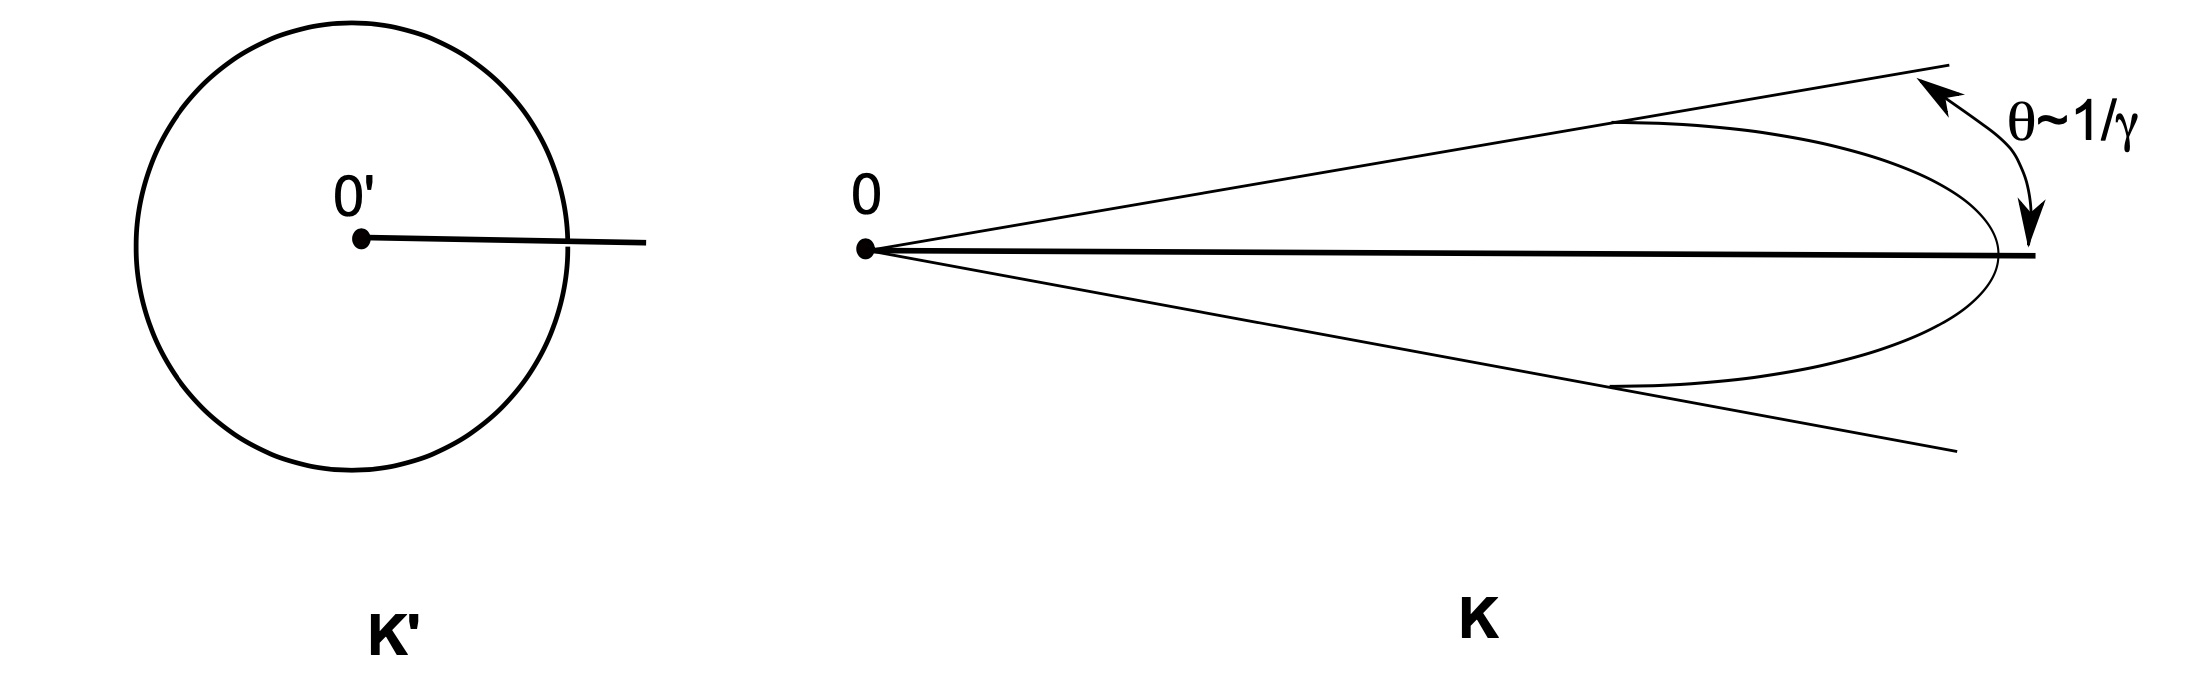
\includegraphics[width=0.8\textwidth]{aberration.jpg}
\caption{aberration}
\end{figure}

A photon emitted at \( \theta^\prime = 0 \) in the primed frame travels at \( \theta = 0 \) in the observer's frame. Conversely, a photon emitted at \( \theta^\prime = \frac{\pi}{2} \) travels at an angle \( \theta \) approximated by \( \theta \simeq \frac{1}{\gamma} \).

This indicates that emission isotropic at the source is not perceived as isotropic by an observer if there is a relativistic boost between them. This is particularly relevant for phenomena like gamma-ray bursts (GRBs), which are strongly beamed in the forward direction, forming a cone with an opening angle of approximately \( \sim \frac{2}{\gamma} \).

In the non-relativistic limit, the frequency of the emitted radiation corresponds to the gyro-frequency, leading to a mono-chromatic spectrum at this frequency.

However, in the relativistic regime, continuous emission is altered by the beaming effect. The signal is visible only at specific angles due to this effect. The resulting spectrum is still a Fourier transform of the time-dependent emission, but now it has a characteristic timescale \(  \Delta t \), giving a frequency spectrum peaked around \( \sim \frac{1}{\Delta t} \).

\begin{figure}[t]
\centering
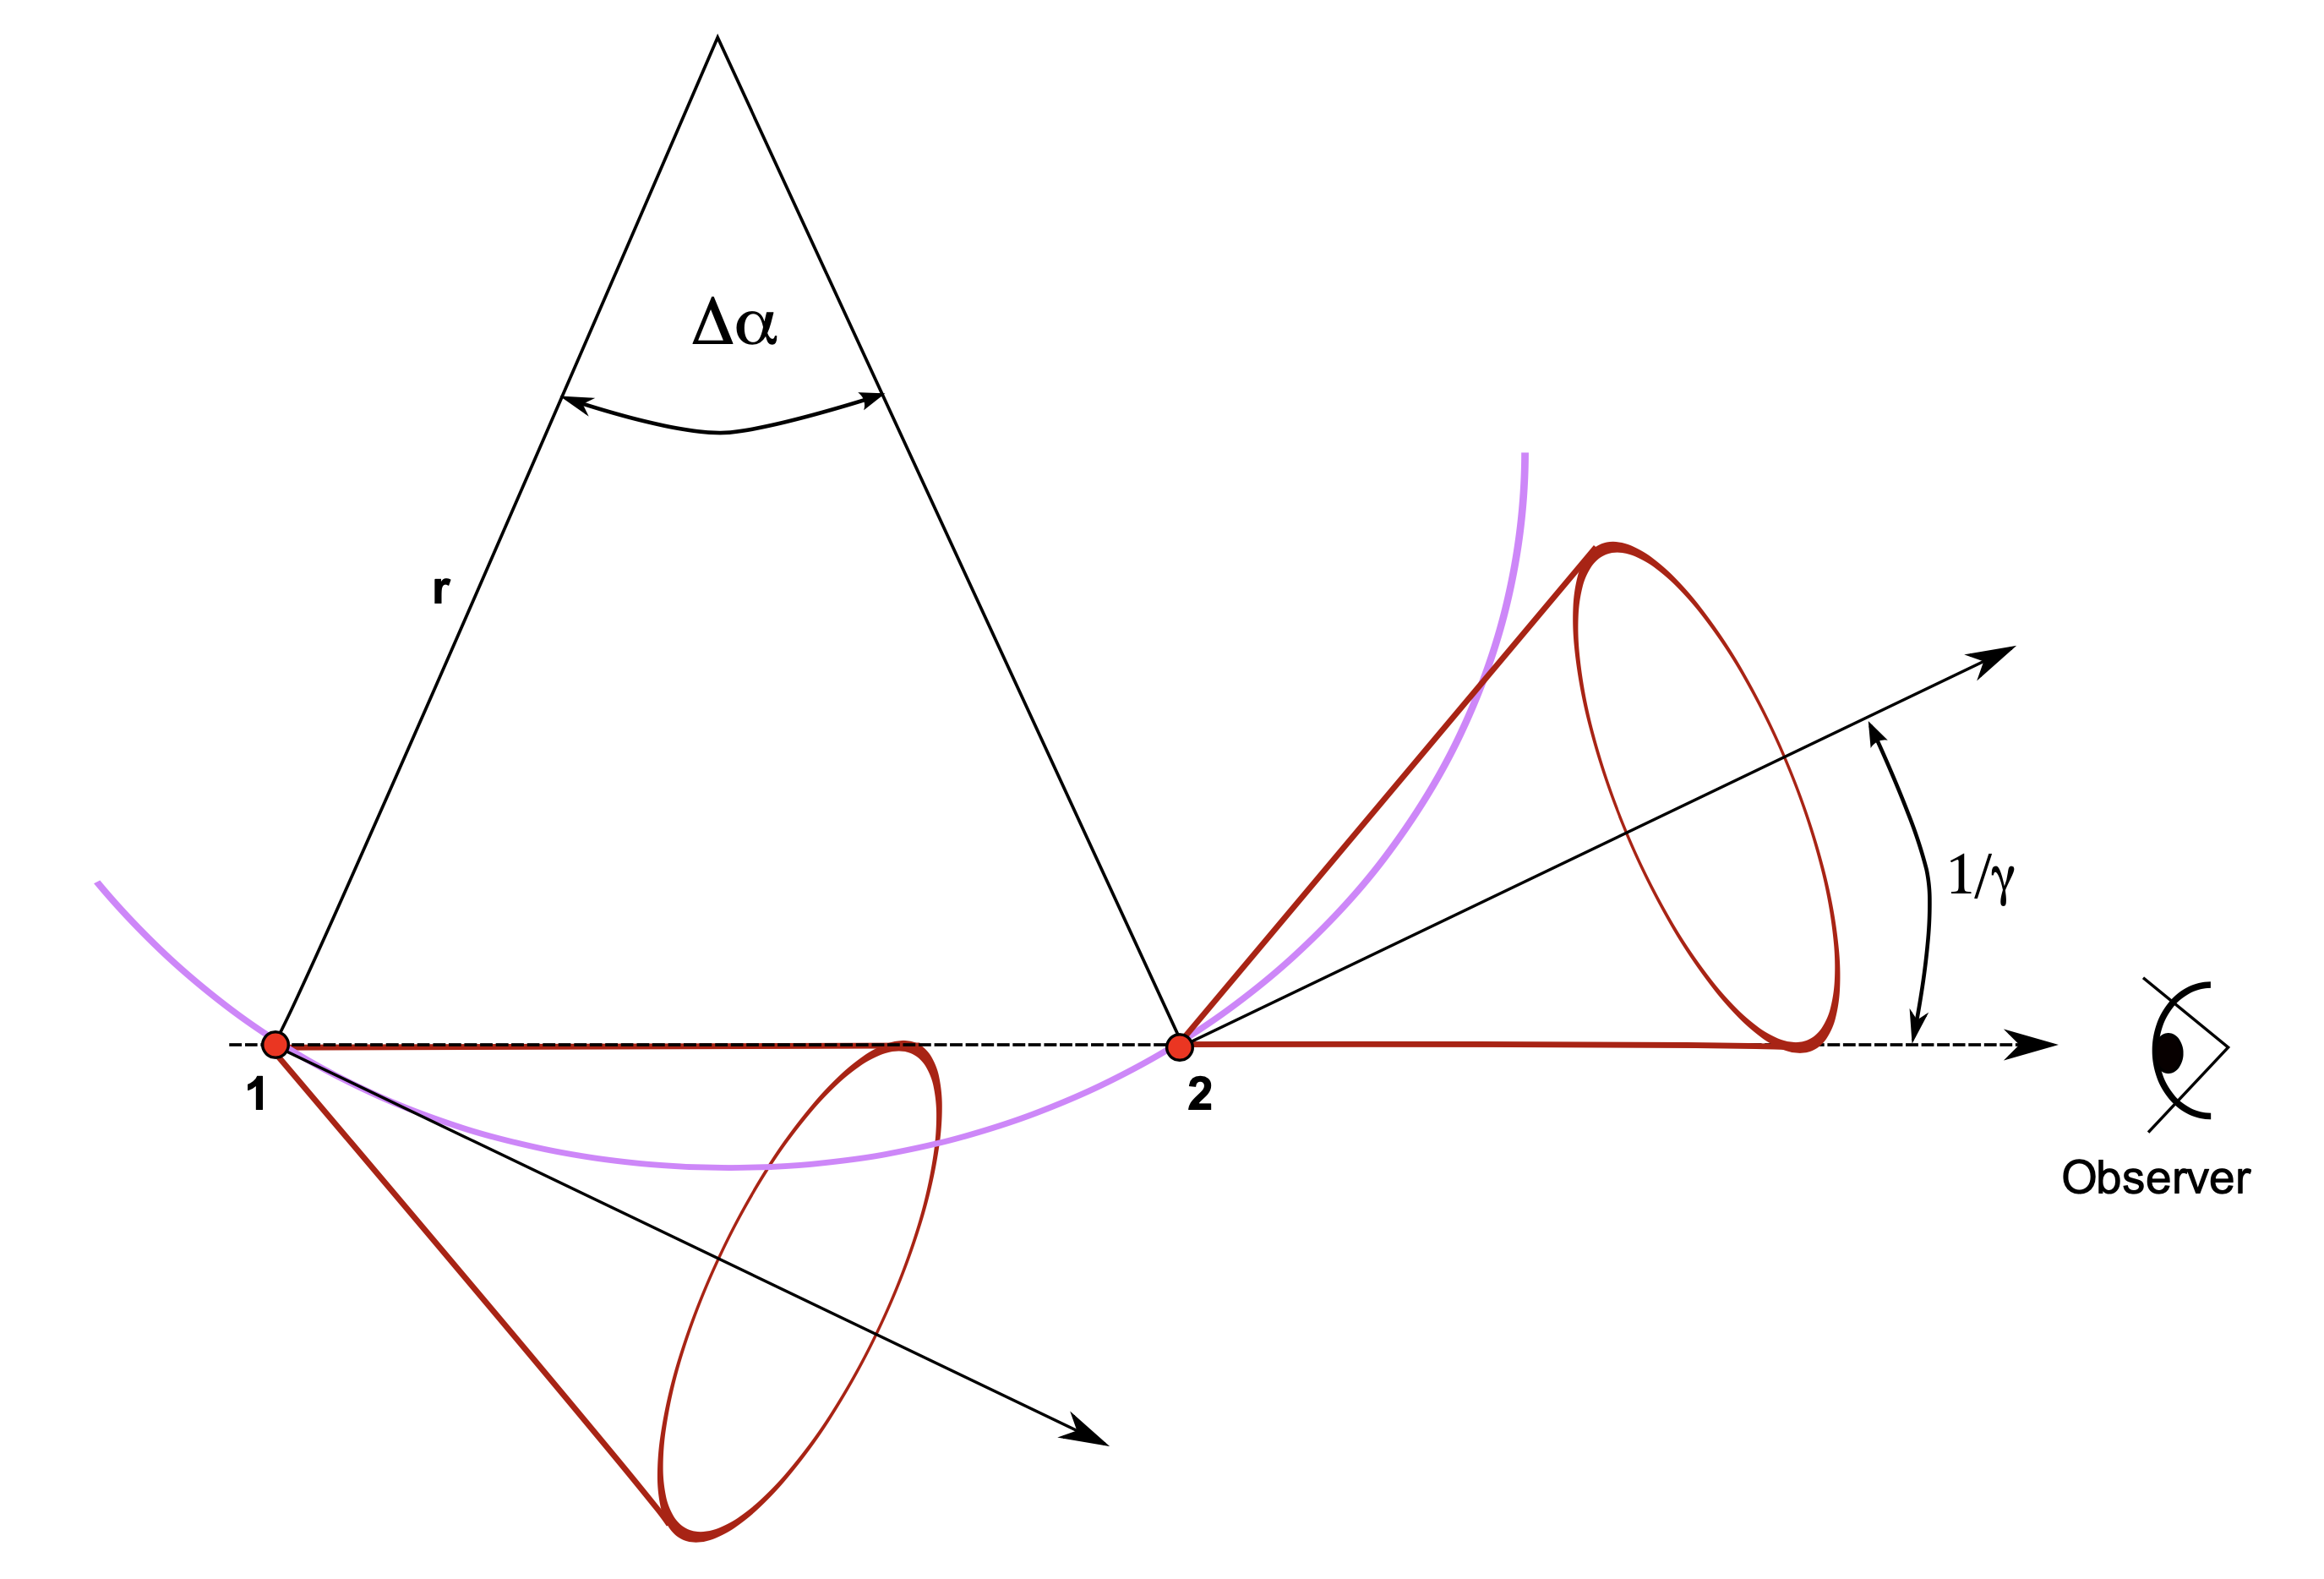
\includegraphics[width=0.8\textwidth]{opening.png}
\caption{opening}
\end{figure}

To determine the duration of emission as perceived by a distant observer, consider the time taken for an electron to move from point A to B. This segment of the trajectory corresponds to the period during which the radiation emitted by the electron falls within the observer's view because of the emitted cone:
%
\[
\Delta t = \frac{\text{AB}}{v}
\]

At the observer ($\delta t_i$ is the time for the \emph{photon} to reach the observer): 
%
\[
\Delta t_{\rm obs} = t_B + \delta t_B - (t_A  + \delta t_A) = (t_B - t_A) + (\delta t_B - \delta t_A) = \frac{\text{AB}}{v} - \frac{\text{AB}}{c} = \frac{\text{AB}}{v} (1-\beta)
\]

Using AB~$= \frac{2}{\gamma}r_{\rm L}$, we get:
%
\[
\Delta t_{\rm obs} = \frac{\text{AB}}{v} (1-\beta) \frac{1+\beta}{1+\beta} \overset{\beta \sim 1}{\simeq} \frac{\text{AB}}{v} \frac{1}{2\gamma^2} \simeq {\color{red}\frac{r_{\rm L}}{\gamma^3}}
\]

An observer sees a sequence of pulses of width:
%
\[
\Delta t_{\rm obs} \simeq \frac{1}{v \gamma^2 \nu_g} %\simeq \frac{1}{\gamma^3 \nu_L} 
\]

These pulses are separated by a gyration time 
%
\[
T \simeq \frac{1}{\nu_L} = \frac{\gamma}{\nu_g}
\]

\begin{figure}[t]
\centering
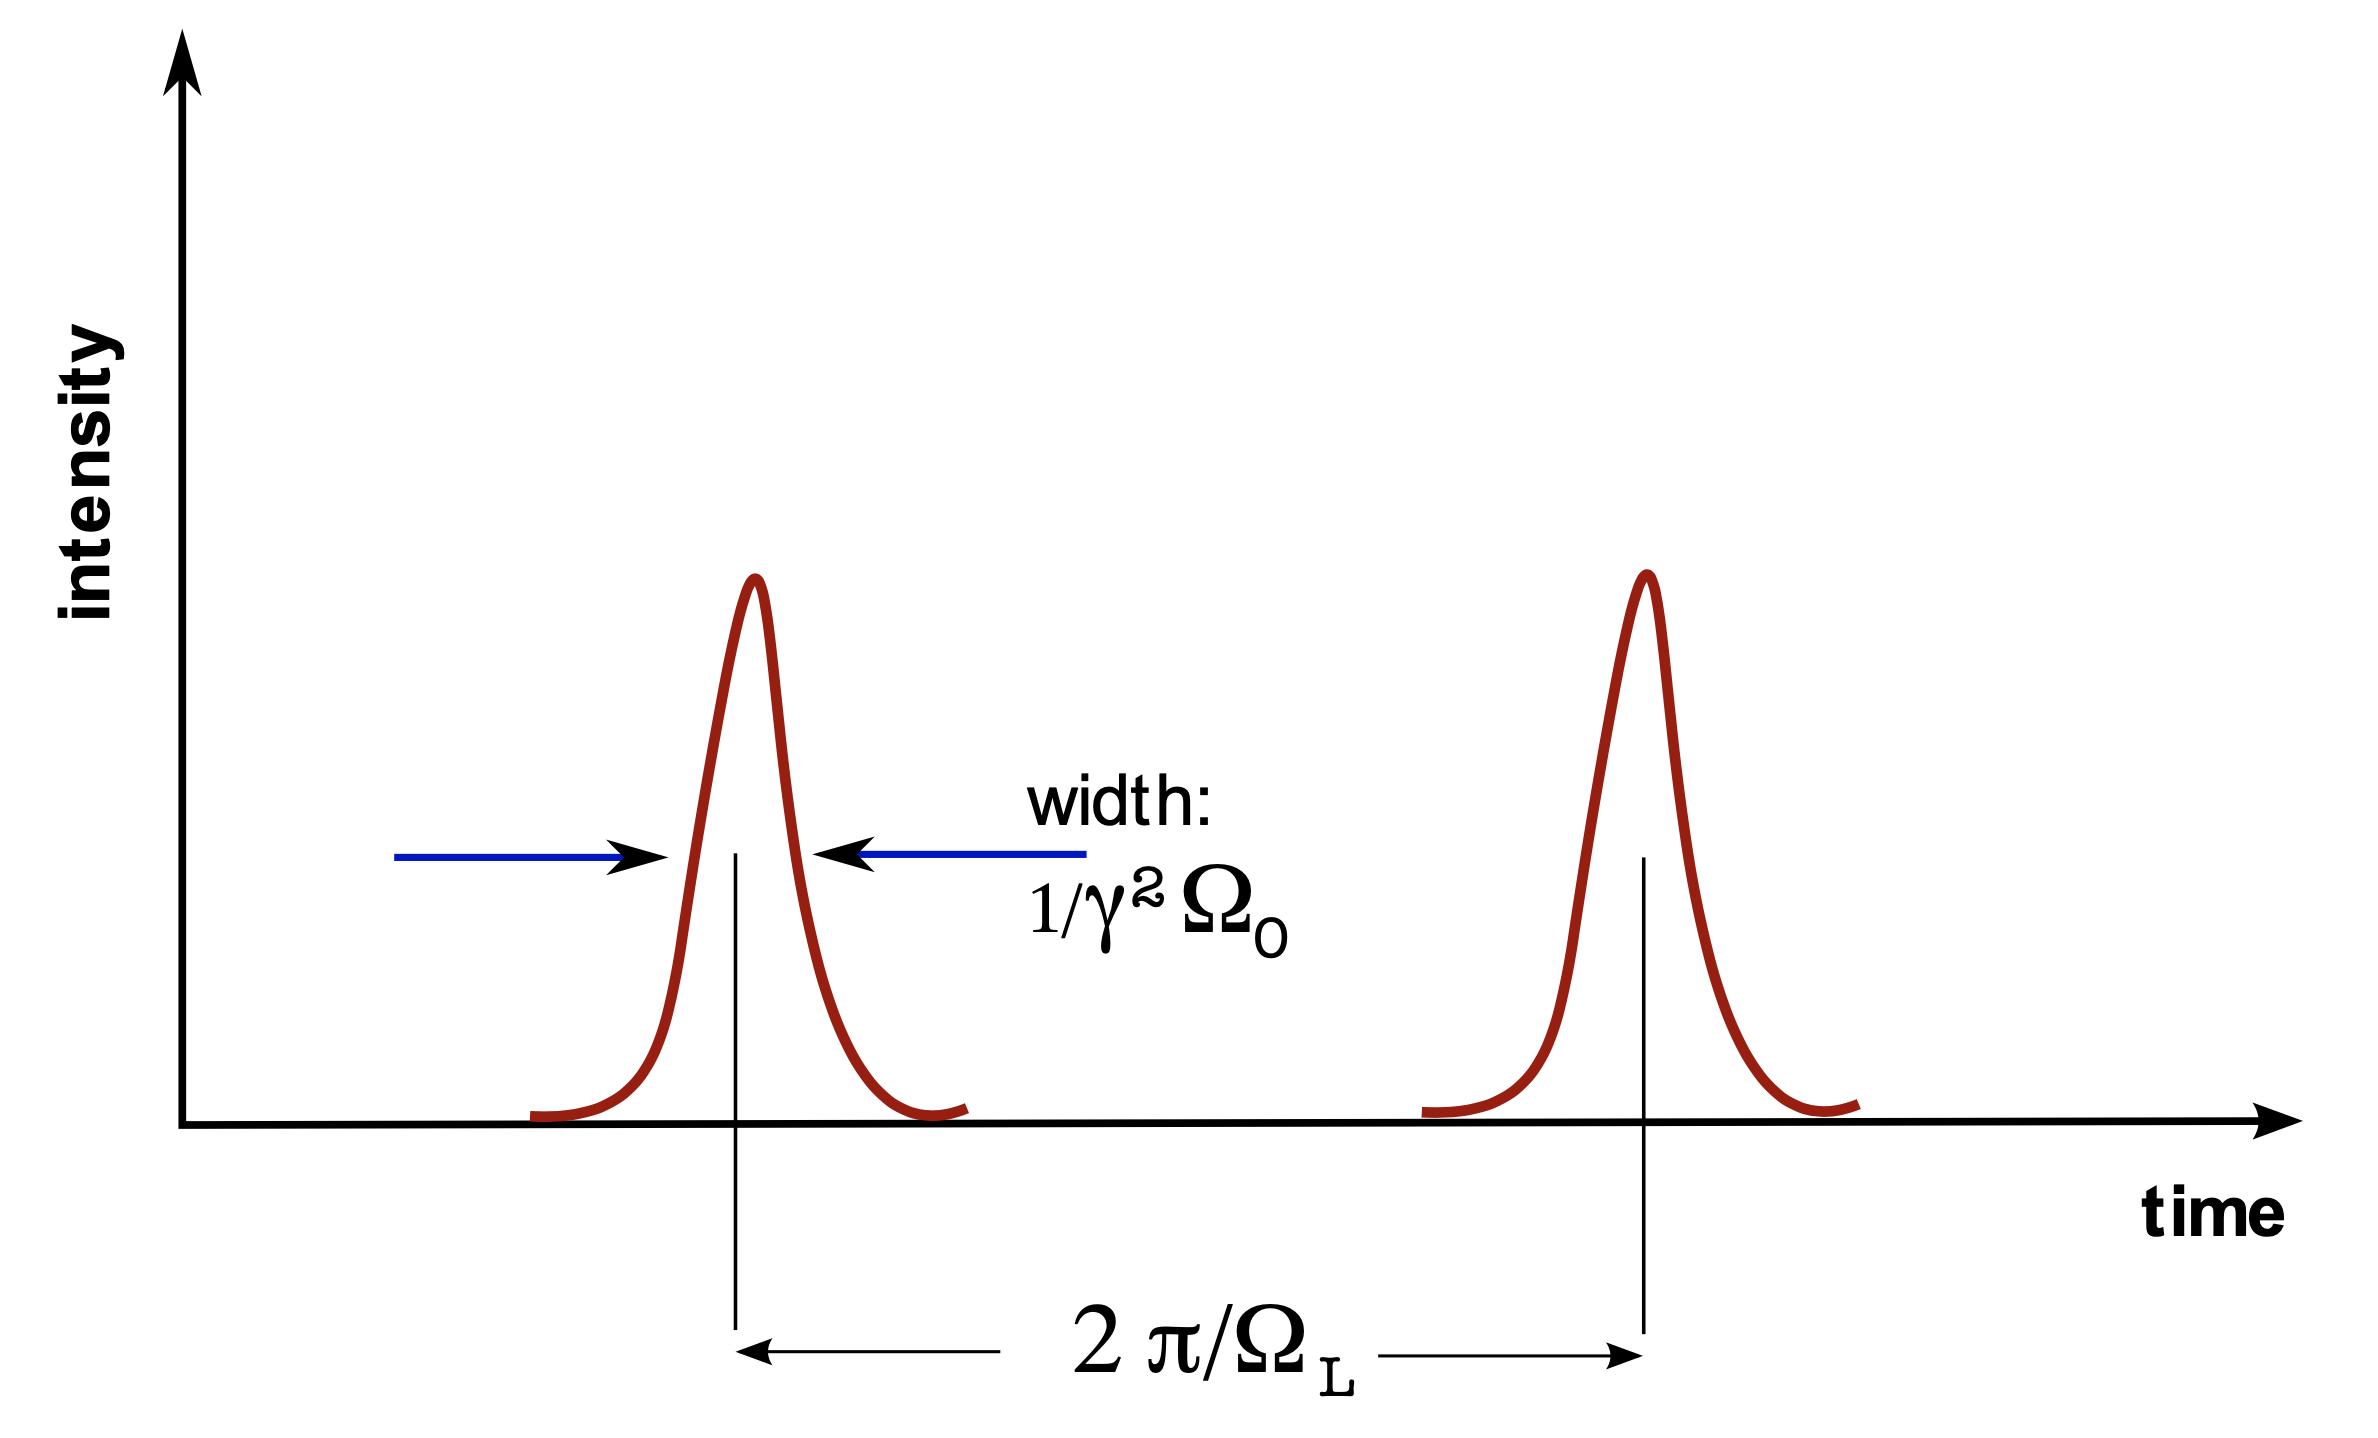
\includegraphics[width=0.8\textwidth]{observedelectricfield.png}
\caption{observedelectricfield}
\end{figure}

Thus, in the relativistic limit, the spectrum experiences a \( \gamma^2 \) boost compared to the cyclotron frequency:
%
\begin{remark}
\[
\nu_s \sim \frac{1}{\Delta t_{\rm obs}} = \frac{\gamma^3}{r_{\rm L}} = \gamma^2 \nu_g
\]
\end{remark}

\begin{problem}
Compute the properties of the Galactic radio emission.
\end{problem}

The full result for a single electron with Lorentz factor \( \gamma \) is:
%
\[
P_\nu(\nu, \gamma, \theta) = \frac{\sqrt 3 q^3 B}{m_e c^2} \sin \theta F\left(\frac{\nu}{\nu_c}\right)
\]
%
where $P_\nu$ is the power per \emph{unit of frequency}, the characteristic frequency $\nu_c = \frac{3}{4\pi} \gamma^2 \frac{qB}{m_e c} \sin \theta$, and the synchrotron function is
%
\[
F(x) = x \int_x^\infty K_{5/3} (x^\prime) dx^\prime
\]

A useful approximation for \( P_\nu \) is 
%
\[
P_\nu \simeq 1.8 \left(\frac{\nu}{\nu_c}\right)^{1/3} \exp\left(-\frac{\nu}{\nu_c}\right)
\]
%
notice that the \emph{peak} frequency is approximately  \( \nu_{\rm max} \simeq 0.29 \nu_c \).

\subsection{Quantum correction}

In our previous analysis of synchrotron radiation, we assumed that the motion of electrons does not change significantly due to photon emission. However, considering that photons carry momentum, there should be some recoil effect on the emitting electron. This aspect becomes particularly relevant when the energy of the emitted synchrotron photon, \( h \nu_s \), approaches the electron's relativistic energy, \( \gamma m_e c^2 \). Given that \( \nu_s \propto \gamma^2 \), this effect is more pronounced at higher energies.

To quantify this, we introduce the parameter \( \chi \):
%
\[
\chi = \frac{B}{B_q}\frac{p}{mc} \sim \frac{h\nu_s}{\gamma mc^2}
\]

Here, \( p \) is the electron momentum, and \( B_q = \frac{m^2 c^3}{e \hbar} \approx 4.4 \times 10^{13} \) G is a characteristic magnetic field strength.

For \( \chi \ll 1 \), the motion can be considered Newtonian, while for \( \chi \gg 1 \), quantum effects dominate. In extremely strong magnetic fields, like those found in pulsar atmospheres (\( \sim 10^{15} \) G), quantum effects become significant even for relatively low electron momenta.

According to Landau, the power radiated in the quantum regime (\( \chi \gg 1 \)) is:
%
\[
P_q \propto \frac{e^2 m^2 c^3}{\hbar^2} \left( \frac{B}{B_q}\right)^{2/3} \gamma^{2/3}
\]

This indicates that the power dependency shifts from \( \gamma^2 \) to \( \gamma^{2/3} \) in the quantum regime.

The spectrum in this regime peaks broadly and almost flatly around a frequency that satisfies:
%
\[
\frac{h\nu}{E - h\nu} \sim \chi
\]

For \( \chi \ll 1 \), the emitted frequency \( \nu \) is approximately equal to the synchrotron frequency \( \nu_s \). In contrast, for \( \chi \gg 1 \), \( h\nu \) is comparable to the initial energy \( E \), indicating that the emitted photon carries away a significant portion of the electron's energy. This results in catastrophic energy losses and a non-continuous process, necessitating a \emph{Monte Carlo} approach for accurate modeling.

\subsection{Synchrotron emission by an electron population}

Assume to have a population of electrons with a power-law distribution in energy within some given range:
%
\[
n(\gamma) d\gamma = n_0 \gamma^{-p} d\gamma \quad \gamma_{\rm min} < \gamma < \gamma_{\rm max} 
\]	
%
where $n(\gamma) d\gamma$ is the electron volume density, and usually the slope is $p \sim 2-3$.

The specific emissivity is given by
%
\begin{equation*}
j_\nu = \int_1^\infty \langle P_\nu(\gamma) \rangle n(\gamma) d\gamma
\end{equation*}
%
where $P_\nu$ is the power emitted per unit frequency.

We simplify our calculations assuming a $\delta$-function for $P_\nu$:
%
\begin{equation*}
P_\nu(\gamma) \simeq \langle P_s \rangle \delta(\nu - \nu_c)
\end{equation*}
%
follows
%
\begin{equation*}
j_\nu = \frac{4}{3} c \sigma_{\rm T} U_{\rm B} n_0 \int_{\gamma_{\rm min}}^{\gamma_{\rm max}} \gamma^{2-p} \delta(\nu - \gamma^2 \nu_{\rm L}) d\gamma
\end{equation*}
%
finally
%
\begin{remark}
\[ 
j_\nu = \frac{2}{3} c \sigma_{\rm T} n_0 \frac{U_{\rm B}}{\nu_{\rm L}} \left( \frac{\nu}{\nu_{\rm L}} \right)^{\color{red}-\frac{p-1}{2}}
\]
\end{remark}
%
which is valid in the range $\gamma^2_{\rm min} \nu_{\rm L} < \nu < \gamma^2_{\rm max} \nu_{\rm L}$

%\begin{center}
%\includegraphics[scale=0.18]{figures/synchropowerlaw.png}
%\end{center}

Outside the validity limits we have to use the complete expression and we obtain 
%
\begin{equation*}
j_\nu \propto \nu^{1/3} \quad\text{ for }\quad \nu < \nu_{\rm min}
\end{equation*}
%
and
%
\begin{equation*}
j_\nu \propto \exp \left(-\frac{\nu}{\nu_{\rm max}}\right) \quad\text{ for }\quad \nu > \nu_{\rm max}
\end{equation*}

\subsection{Kinetic equation for electron evolution}

TO BE DONE

\subsection{Synchrotron Self-Absorption}

The Synchrotron self-absorption corresponds to the inverse process where a free electron can absorb a synchrotron photon in a magnetic field $e+B+\gamma\rightarrow e+B$.

We provide here an heuristic derivation of how this process impacts on the spectrum. In fact, we have a population of electrons which are emitting radiation and absorbing radiation and we want to compute the intensity using the radiative transfer equation.

Let's remind that for a thermal distribution of electrons, the source function would correspond to the black-body
%
\[
S_\nu = {\color{red}\left(\frac{2\nu^2}{c^2}\right)} {\color{blue}\left(\frac{h\nu}{\exp(h\nu / kT) - 1}\right)} 
\propto {\color{red}\nu^2} {\color{blue}\langle E \rangle}
\]
%
where the first term is the \emph{phase-space factor} and the second is the \emph{mean electron energy} emitting photons at frequency $\nu$.

In fact, in the Rayleigh-Jeans limit $kT \gg h\nu$ and
%
\[
\langle E \rangle \simeq kT \lim_{x\rightarrow 0} \frac{x}{\exp x - 1} \sim kT
\]

For a non-thermal synchrotron radiation $kT$ must be replaced by the mean energy of an electron emitting synchrotron radiation at frequency $\nu$
%
\begin{equation*}
\nu \simeq \gamma^2 \nu_{\rm L} \rightarrow \gamma \sim \left(\frac{\nu}{\nu_{\rm L}}\right)^{1/2}
\end{equation*}
%
follows
%
\begin{equation*}
S_\nu \sim \left( \frac{2\nu^2}{c^2} \right) \gamma m_e c^2
\propto \left( \frac{2\nu^2}{c^2} \right) \left(\frac{\nu}{\nu_{\rm L}}\right)^{1/2} 
\propto B^{-1/2} \nu^{5/2} 
\end{equation*}

%\begin{center}
%\includegraphics[scale=0.06]{figures/x299.png}
%\end{center}

From the definition of the source term \( S_\nu = \frac{j_\nu}{\alpha_\nu} \), follows
%
\[
\alpha_\nu = \frac{j_\nu}{S_\nu} 
\propto (B^{\frac{p+1}{2}} \nu^{-\frac{p-1}{2}}) (B^{\frac 1 2} \nu^{-\frac 5 2})
= B^{\frac{p+2}{2}} \nu^{-\frac{p + 4}{2}}
\]

We notice that $\alpha_\nu$ decreases towards higher frequencies, so it will be relevant at low energies.

From the transfer equation $I_\nu = S_\nu [1 - \exp(-\tau_\nu)]$ and reminding $\tau_\nu = \alpha_\nu s$, we identify the following limiting regimes:
%
\begin{itemize}
\item for $\tau_\nu \gg 1$ corresponding to small frequencies $I_\nu \rightarrow S_\nu$

\item for $\tau_\nu \ll 1$ corresponding to large frequencies $I_\nu \rightarrow S_\nu \alpha_\nu s = j_\nu s$
\end{itemize}

Therefore for each source exists a frequency $\nu_B$ where $\tau_B = 1$ and the corresponding spectrum will be:
%
\begin{itemize}
\item for $\nu \ll \nu_B$ (optically thick) and $I_\nu \propto \nu^{5/2}$, notice independent on $p$!

\item for $\nu \gg \nu_B$ (optically thin) and $I_\nu \propto \nu^{-\frac{p-1}{2}}$
\end{itemize}

% TYPICAL SPECTRUM OF A RADIO SOURCE

\begin{problem} Estimate the age of the source from the break.
\end{problem}

%As our observing frequency increases, we see photons coming from regions of the source that are progressively deeper and deeper, and as we do so the total flux density increases. However, of course, eventually we reach a point where we can “see all the way through” the plasma, and above this frequency we recover the underlying power-law distribution.

%\begin{center}
%\includegraphics[scale=0.14]{figures/selfabsorption.png}
%\end{center}

%Representative spectra of \textbf{radio galaxies and quasars}. The radio source 3C 84 in the nearby galaxy NGC 1275 contains a very compact nuclear component that is opaque below about 20 GHz. The radio galaxy 3C 123 is transparent at all plotted frequencies, and energy losses steepen its spectrum above a few GHz. The quasar 3C 48 is synchrotron self-absorbed only below 100 MHz, while the quasar 3C 454.3 contains structures of different sizes that become opaque at different frequencies.

\subsection{Minimum Energy and Equipartition}

The existence of a synchrotron source implies the presence of relativistic electrons with some energy density $U_{\rm e}$ and a magnetic field whose energy density is $U_{\rm B} = \frac{B^2}{8\pi}$. 
%
What is the \emph{minimum total energy in relativistic particles and magnetic fields} required to produce a synchrotron source of a given radio luminosity?

The energy density in particles is
%
\[
U_e = \int_{\gamma_{\rm min}}^{\gamma_{\rm max}} E n(\gamma) d\gamma
%\simeq n_0 m_e c^2 \int_{\gamma_{\rm min}}^{\infty} \gamma^{1-p} d\gamma n_0 m_e c^2 = \frac{n_0 m_e c^2}{p-2} \gamma_{\rm min}^{-(p-2)}
\]
%
and the corresponding luminosity is
%
\[
\mathcal L = V \int_{\gamma_{\rm min}}^{\gamma_{\rm max}} \left| \frac{dE}{dt} \right| n(\gamma) d\gamma
%\simeq n_0 m_e c^2 \int_{\gamma_{\rm min}}^{\infty} \gamma^{1-p} d\gamma n_0 m_e c^2 = \frac{n_0 m_e c^2}{p-2} \gamma_{\rm min}^{-(p-2)}
\]

For a power-law distribution $n(\gamma) \propto \gamma^{-p}$, and using $P \propto \gamma^2 U_B$ the ratio between the two is proportional to
%
\begin{equation*}
\frac{U_e}{\mathcal L} \propto \frac{1}{U_B} \frac{\int_{\gamma_{\rm min}}^{\gamma_{\rm max}} \left( \frac{\gamma}{\gamma_{\rm min}}\right)^{1-p} d\gamma}{\int_{\gamma_{\rm min}}^{\gamma_{\rm max}}  \left( \frac{\gamma}{\gamma_{\rm min}}\right)^{2-p}  d\gamma} \propto \frac{1}{U_B} \frac{\gamma_{\rm min}^{2-p}}{\gamma_{\rm min}^{3-p}} \propto \frac{1}{U_B \gamma_{\rm min}}
\end{equation*}	

Finally, $\nu_s \propto \gamma^2 B$ therefore $\gamma \propto B^{-1/2}$, for a fixed frequency, and thereby $U_e / \mathcal L \propto B^{-3/2}$.  

We conclude that the electron energy density needed to produce a given synchrotron luminosity scales as $U_e \propto B^{-3/2}$. % while the magnetic energy density $U_B \propto B^2$.

The minimum of the total energy density $U$ as a function of $B$ occurs at
%
\begin{equation*}
\frac{dU}{dB} = \frac{d}{dB} (U_e + U_B) = 0 \rightarrow \frac{-3/2}{B} U_e + \frac{2}{B} U_B = 0
\end{equation*}

The ratio of cosmic-ray particle energy density to magnetic field energy that minimizes the total energy is
%
\begin{remark}
\[
\frac{U_e}{U_B} = \frac{4}{3}
\]
\end{remark}

This ratio is nearly unity, so minimum energy constraint for an optically thin synchrotron source places similar amount of energy in particles as in magnetic fields (equipartition).

\begin{problem}
Cygnus A (3C 405)
\end{problem}

%Physical motivated.

\section{Inverse Compton Scattering}

The IC process involves the up-scattering of background photons by high-energy (HE) electrons (\(e + \gamma \rightarrow e' + \gamma'\)). It is a significant energy loss mechanism for electrons if their energy exceeds that of the photons.

To derive the power emitted during IC scattering, we initially approach from a classical perspective before discussing quantum interpretations.

In the classical view, an electromagnetic wave strikes an electron, causing it to oscillate and thus radiate power due to acceleration. The Poynting flux (\( \vb S \)) of a plane wave incident on an electron is:
%
\[
\vb S =  \frac{c}{4\pi} \vb E \times \vb B \rightarrow S = \frac{c}{4\pi} | \vb E |^2   
\]

The Lorentz force acting on the electron is:
%
\[
\vb F = q (\vb E + \frac{\vb v}{c} \times \vb B) \simeq q \vb E
\]
%
assuming \( | \vb v | \ll c \).

The oscillating electric field of the wave is:
%
\[
\vb E = E_0 \vb \epsilon \sin (\omega t + \phi)
\]
%
leading to an average acceleration:
%
\[
\vb a = \frac{\vb F}{m} \rightarrow \langle a^2 \rangle = \frac{q^2}{m^2} \frac{E_0^2}{2}
\]
%
where we used
%
\[
\frac{1}{T} \int_0^{T = \frac{2\pi}{\omega}} \sin^2 (\omega t) dt = \frac{1}{2}
\]

Thus, the average power radiated by the electron is:
%
\[
\langle P \rangle = \frac{2}{3} \frac{q^2 a^2}{c^3} = \frac{2}{3} \frac{q^2}{c^3} \frac{a^2}{m^2} \frac{E_0}{2} = \frac{1}{3} \frac{q^4}{m^2 c^3} E_0^2
\]

The classical cross-section associated to this process is the \emph{ratio} between the power radiated and the impinging flux
%
\begin{remark}
\begin{equation*}
\langle P \rangle = \sigma_{\rm T} \langle | \vb S | \rangle \rightarrow \sigma_{\rm T} = \frac{1}{3} \frac{q^4}{m^2 c^3} E_0^2 \frac{8\pi}{c} \frac{1}{E_0^2} = \frac{8}{3} \pi \left( \frac{q^2}{m c^2} \right)^2
\end{equation*}
\end{remark}
%
where we use the average Poynting flux $\langle \vb S \rangle = \frac{c}{8\pi} E_0^2$.

This is known as Thomson cross-section and its numerical value is 
%
\begin{equation*}
\sigma_{\rm T} \simeq 6.652 \cdot 10^{-25}~\text{cm}^2
\end{equation*}

In other words, the electron will extract from the incident radiation the amount of power flowing through the area $\sigma_T$ and reradiate that power over the doughnut-shaped pattern given by Larmor’s equation.

%The classical cross-section associated with this process, known as the Thomson cross-section, is:
%\[
%\sigma = \frac{8}{3} \pi \left( \frac{q^2}{m c^2} \right)^2
%\]

%This implies the electron extracts and reradiates power from the incident radiation flowing through an area equal to the Thomson cross-section (\( \sigma_{\rm T} \)).

The time-averaged scattered power by a single particle is:
%
\[
P = \sigma_{\rm T} c U_{\rm rad}
\]
%
where \( U_{\rm rad} = S /c \) is the energy density of the incident radiation.

Incidentally, the Thomson optical depth, representing the probability of a photon undergoing Thomson scattering (notice this is the opposite process!) is:
%
\[
\tau_e = \int n_e \sigma_{\rm T} ds
\]

\begin{problem}
The Intergalactic Medium (IGM) at redshifts \( z \lesssim 10 \) is observed to be highly ionized, likely due to radiation from galaxies and quasars. Post-recombination at \( z \approx 10^3 \), the IGM was almost completely neutral. This observation indicates that reionization of the IGM occurred somewhere \( z_r \gtrsim 10 \), although the exact timing of this crucial transition remains unknown. 

An ionized IGM Thomson scatters CMB photons. Under the assumption of a uniform Universe with a specified baryon fraction \( \Omega_b \) in units of the critical density \( \Omega_c \), derive the relation between \( \tau_r \) and \( z_r \) and calculate \( \tau_r \) assuming a reionization redshift \( z_r = 10 \) for an Einstein-de Sitter Universe.
\end{problem}

The Compton scattering process, involving the interaction of photons with electrons, can be effectively described using quantum mechanics.

We start by imposing the energy and momentum balance in the scattering process:
%
\[
K_i^\mu + P_i^\mu = K_f^\mu + P_f^\mu
\]
%
where \( P_{i,f}^2 = m_e^2 \) and \( K_{i,f}^2 = 0 \) (for photons).

Contracting the final momentum gives:
%
\[
 P_f^\mu P_{f \mu} = (P_i + K_i - K_f)^\mu (P_i + K_i - K_f)_\mu  \rightarrow m_e^2 = m_e^2 + 2 (P_i K_i - P_i K_f - K_i K_f)
\]

In the frame where the electron is initially at rest \( P_i = \left( m_e, \vb 0 \right) \), and assuming the x-axis is aligned with the incoming photon, we have:
%
\[
K_i = \epsilon_i (1, 1, 0, 0) \quad \text{and} \quad K_f = \epsilon_f (1, \cos \theta, \sin \theta, 0)
\]

Substituting these into the equation, we get:
%
\[
m_e^2 = m_e^2 + 2 \left( m_e \epsilon_i - m_e \epsilon_f - \epsilon_i \epsilon_f + \epsilon_i \epsilon_f \cos \theta \right)
 \rightarrow m_e (\epsilon_i - \epsilon_f) = \epsilon_i \epsilon_f (1-\cos\theta)    
\]

Leading to the relation for the final photon energy:
%
\begin{remark}
\[
\epsilon_f = \frac{\epsilon_i}{1+ \frac{\epsilon_i}{m_e c^2} (1-\cos\theta)}
\]
\end{remark}

The fractional energy change of the photon is:
%
\[
\frac{\Delta \epsilon}{\epsilon}  
= \frac{\epsilon_f - \epsilon_i}{\epsilon_i} = -1 + \frac{1}{1 + \frac{\epsilon_i}{m_e c^2} (1-\cos\theta)} \overset{\epsilon_i \ll m_e c^2}{\longrightarrow} - \frac{\epsilon_i}{m_e c^2} (1-\cos\theta)
\]

This equation describes \emph{Compton scattering}, where a photon scatters off an electron and transfers energy, resulting in a decrease in photon energy. Notably, unless the photon's energy is comparable to or larger than the electron mass in the electron's rest frame, the photon energy is only slightly altered.

Thomson scattering accurately describes the regime where the incident photon energy \( \epsilon_i \) is much less than the electron rest energy (\( \epsilon_i \ll m_e c^2 \)). In this regime, energy transfer is minimal, \( \epsilon_i \simeq \epsilon_f \), indicative of quasi-elastic scattering.

However, as \( \epsilon_i \) approaches or exceeds \( m_e c^2 \), the energy transfer becomes significant, marking a transition to deeply inelastic scattering. This regime is governed by the Klein-Nishina (KN) cross-section.

The full Klein-Nishina cross-section, derived using Quantum Electrodynamics (QED), is given by:
%
\[
\sigma_{\rm KN} = \frac{3}{4} \sigma_{\rm T} \left[ \frac{1+x}{x^3} \left(\frac{2x(1+x)}{1+2x} - \ln (1+2x)\right) + \frac{1}{2x} \ln (1+2x) - \frac{1+3x}{(1+2x)^2} \right]
\]
%
where \( x = \epsilon_i / m_e c^2 \).

In the limit of \( x \ll 1 \), the equation converges to the Thomson limit \[ \sigma(x) \simeq \sigma_{\rm T} (1-2x+\dots) \] while in the extreme KN limit (\( x \gg 1 \)), it approaches \[ \sigma(x) \simeq \frac{3}{8} \sigma_{\rm T} \frac{1}{x} (\ln 2x + \frac{1}{2}) \]

Therefore, the principal effect of the KN regime is a reduction in the cross-section relative to the classical Thomson value as the photon energy increases.

%%% PLOT

When the electron involved in Compton scattering has a velocity \( \beta \) in the laboratory (LAB) frame, the scattering dynamics change.

The relationship in the electron's rest frame (primed frame) remains valid:
%
\[
\epsilon^\prime_f = \frac{\epsilon^\prime_i}{1+ \frac{\epsilon^\prime_i}{m_e c^2} (1-\cos\theta^\prime)}
\]
%
where \( \theta^\prime \) is the angle between incoming and outgoing photon directions in the primed frame. Applying Lorentz transformation:
%
\[
\epsilon'_i = \epsilon_i \gamma (1-\beta \cos \alpha)
\]
%
where \( \alpha \) is the angle between the photon and electron in the LAB frame.

To express \( \epsilon^\prime_f \) in the LAB frame and account for the emission angle \( \alpha^\prime \) in the comoving frame:
%
\[
\epsilon_f = \gamma(1+\beta \cos\alpha^\prime) \epsilon^\prime_f = 
\gamma (1+\beta \cos \alpha^\prime) \frac{\epsilon^\prime_i}{1+ \frac{\epsilon^\prime_i}{m_e c^2} (1-\cos\theta^\prime)}
\]
%
or
\[
\epsilon_f = \gamma^2 \epsilon_i \frac{(1+\beta \cos\alpha^\prime)(1-\beta \cos\alpha)}{1+ \frac{\epsilon^\prime_i}{m_e c^2} (1-\cos\theta^\prime)}
\]

In the limit \( \epsilon_i \ll m_e \) (or equivalently \( \gamma \epsilon_i \ll m_e c^2 \) or \( E_e \epsilon_i \ll m_e^2 c^4 \) in the LAB frame):
%
\[
\epsilon_f \simeq \gamma^2 \epsilon_i (1+\beta \cos\alpha^\prime)(1-\beta \cos\alpha)
\]

For isotropic incident and outgoing radiation in the electron's comoving frame, the average final energy is approximately 
%
\begin{remark}
\[
 \epsilon_f \simeq \gamma^2 \epsilon_i \simeq 30 \left(\frac{\epsilon_i}{\rm eV}\right)\left(\frac{E_e}{\rm GeV}\right)^2 \, \text{MeV}   
\]
\end{remark}

While the scattering angle is arbitrary in the \emph{comoving} frame, in the LAB frame, the outgoing radiation is \emph{beamed} in the forward direction with an angle \( \frac{1}{\gamma} \).

In the Thomson regime (\( \epsilon^\prime_i \ll m_e \)), the maximum final photon energy, when \( \beta \sim 1 \), \( \cos \alpha^\prime \sim 1 \), and \( \cos \alpha \sim - 1 \), is:
%
\[
\epsilon_{f} \sim 4 \gamma^2 \epsilon_i
\]

In the KN limit, the typical energy of the outgoing photon is:
%
\[
\epsilon_f \simeq \frac{\gamma^2 \epsilon_i}{1 + \frac{\epsilon^\prime_i}{m_e}} \simeq \frac{\gamma^2 \epsilon_i}{\epsilon^\prime_i} m_e \simeq \frac{\gamma^2 \epsilon_i}{\gamma \epsilon_i} m_e \simeq E_e
\]

This implies that in the extreme KN regime, the scattering becomes less frequent, but when it occurs, the scattered photon carries away a significant fraction of the electron's energy.

\begin{remark}
In summary, in the LAB frame:
%
\begin{itemize}
\item In the Thomson regime: \( \epsilon_f \simeq \gamma^2 \epsilon_i \) for \( \gamma \epsilon_i \ll m_e c^2 \)
\item In the KN regime: \( \epsilon_f \simeq \gamma m_e c^2 \) for \( \gamma \epsilon_i \gg m_e c^2 \)
\end{itemize}
\end{remark}

\subsection{Single particle power radiated in IC scattering}

In the Thomson regime, namely $\epsilon'_i \ll m_e c^2$, the power re-emitted by scattering is $\frac{dE}{dt} \simeq \sigma_{\rm T} c U_{\rm rad}$.

We consider now radiation scattering by an ultrarelativistic electron. This expression is still valid in the primed frame instantaneously moving with the electron
%
\begin{equation*}
\frac{dE'}{dt'} = \sigma_{\rm T} c U'_{\rm rad}
\end{equation*}
%
and we want to transform in the LAB frame.

 We recall that the power is LI as it is the ratio of two time-like components, thereby
\begin{equation*}
 \frac{dE}{dt} = \frac{dE'}{dt'} = \sigma_{\rm T} c U'_{\rm rad}
\end{equation*}

The photon density can be seen as the number density of photon of energy $\epsilon$, that is
%
\begin{equation*}
U'_{\rm rad} \simeq 
\int n'_\gamma(\epsilon'_i) \epsilon'_f(\epsilon'_i, \theta) d\epsilon'_i
\end{equation*}
%
where $n'_\gamma(\epsilon') d\epsilon'$ is the number density of incident photons with energy $\epsilon' \rightarrow \epsilon' + d\epsilon'$ \, .

%which is the total power emitted by an electron exposed to some photonfield $n_\gamma(\epsilon)$, 

Similarly, the phase-space distribution is LI as $f (\vb x, \vb p) = \frac{dN}{d^3\vb x d^3 \vb p} = f'(\vb x', \vb p')$, therefore $n(\epsilon) d\epsilon = f d^3 \vb p$ transforms as $d^3 \vb p$ which transforms as an energy, follows
%
\begin{equation*}
\frac{n_\gamma(\epsilon) d\epsilon}{\epsilon} = \frac{n_\gamma(\epsilon') d\epsilon'}{\epsilon'}
\end{equation*}

finally, reminding that in Thomson $\epsilon'_i \simeq \epsilon'_f$ (we are in the electron frame!)

\begin{equation*}
U'_{\rm rad} 
\simeq \int n^\prime_\gamma(\epsilon^\prime_i) {\color{red}\epsilon^\prime_i}  d\epsilon^\prime_i 
= \int \epsilon_i^{\prime 2} \frac{n_\gamma(\epsilon_i)}{\epsilon_i} d\epsilon_i 
% %= \int \epsilon'_i^2 \frac{n'_\gamma(\epsilon'_i)}{\epsilon'_i} d\epsilon'_i 
= \int \epsilon_i^2 \gamma^2 (1-\beta\cos\theta)^2 \frac{n_\gamma(\epsilon_i)}{\epsilon_i} d\epsilon_i 
\end{equation*}

Assuming isotropic incident radiation field
%
\begin{equation*}
\frac{1}{2} \int_{-1}^{1} (1-\beta \cos \theta)^2 d\cos\theta = \frac{1}{2} \int_{-1}^{1} (1-2\beta\cos\theta + \beta^2\cos^2\theta) d\cos\theta = 1 + \frac{\beta^2}{3}
\end{equation*}
%
\begin{equation*}
U'_{\rm rad} = \gamma^2 \left(1 + \frac{\beta^2}{3}\right) U_{\rm rad}
\end{equation*}

therefore the angle-averaged Compton scattered power (in the LAB frame) is
%
\begin{equation*}
\frac{dE}{dt} = \sigma_{\rm T} c U'_{\rm rad} = \sigma_{\rm T} c \gamma^2 \left( 1 + \frac{\beta^2}{3} \right) U_{\rm rad} 
\end{equation*}

We are not done yet! The energy \emph{lost by the electron} and \emph{gained by the photons} is the up-scattered power (power in the final photon field) minus the scattered power (power in the initial photon field)
%
\begin{equation*}
\frac{dE_e}{dt} 
= \sigma_{\rm T} c U'_{\rm rad} - \sigma_{\rm T} c U_{\rm rad}
\end{equation*}

This leads to the IC power as
%
\begin{equation*}
P_{\rm IC} = \sigma_{\rm T} c \left(\gamma^2 +\frac{\gamma^2 \beta^2}{3} -1 \right) U_{\rm rad} = \frac{4}{3}
\sigma_{\rm T} c \beta^2 \gamma^2 U_{\rm rad}
\end{equation*}
%
where I used $\gamma^2 - 1 = \beta^2 \gamma^2$

This is the \emph{net inverse-Compton power gained by the radiation field and lost by the electron}. 

The similarity of the inverse Compton and synchrotron equations shouldn’t be too surprising: they both describe the interaction of an electron with an electromagnetic field.

Note that synchrotron and inverse-Compton losses have the same electron-energy dependence, so their effects on  spectra are indistinguishable.

Dividing by the corresponding synchrotron power 
%
\begin{remark}
\[
\frac{P_{\rm IC}}{P_{\rm s}} = \frac{U_{\rm rad}}{U_{\rm B}}    
\]
\end{remark}
%
which is valid if no absorption and no KN effects are relevant.

What is the average energy increase in the Thomson regime? 

 The number of photons scattered per unit time are
%
\begin{equation*}
\frac{dN_s}{dt} \simeq \frac{\sigma_{\rm T} c U_{\rm rad}}{\langle \epsilon_i \rangle}
\end{equation*}

The average energy increase can be written as
%
\begin{equation*}
P_{\rm IC} \simeq \langle \epsilon_f \rangle \frac{dN_s}{dt} \rightarrow \epsilon_f = \frac{P_{\rm IC}}{dN_s/dt} = \frac{4}{3} \gamma^2 \beta^2 \epsilon_i \simeq {\color{red}\frac{4}{3} \gamma^2 \epsilon_i}
\end{equation*}

If the energy transfer in the K' frame is not neglected (KN regime)
%
\begin{equation*}
- \frac{dE_e}{dt} = P_{\rm IC} = \frac{4}{3} \gamma^2 \beta^2 \sigma_{\rm T} c U_{\rm rad} \left[1 - \frac{63}{10} \frac{\gamma}{m_e c^2} \frac{\langle \epsilon_i^2 \rangle}{\langle \epsilon_i \rangle} + \dots \right]
\end{equation*}
%
where $<\epsilon_i> = \frac{\int \epsilon_i n_\gamma(\epsilon_i) d\epsilon_i}{\int n_\gamma(\epsilon_i) d\epsilon_i}$, which is obtained for incident isotropic photon distribution (see Blumenthal and Gould, 1970).

 Notice that in this regime the photon-field  distribution is relevant (not only the total density as before). 
 
\section{Gamma-ray Absorption}

\begin{figure}[t]
\centering
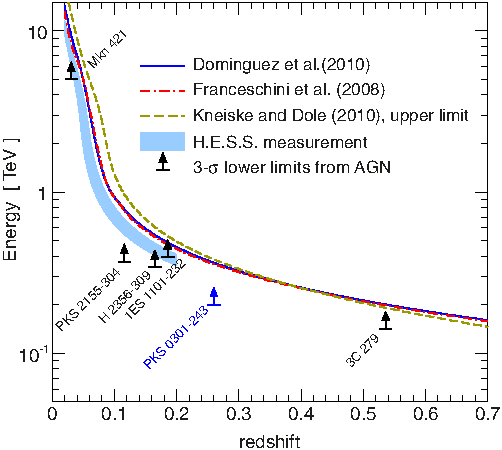
\includegraphics[width=0.5\textwidth]{figures/aa21639-13-fig6.pdf}
\caption{$\gamma$-ray horizon for differen EBL models. Some lower limits from AGN spectra measurements are shown~\cite{HESS2013aa}.}
\end{figure}

Extra-galactic gamma-rays undergo absorption during intergalactic propagation by interacting with photons in the diffuse radiation field, producing electron-positron pairs (\(\gamma + \gamma \rightarrow e^+ + e^-\)). This process depends on the energy threshold condition for opacity.

The square of the center-of-mass (COM) energy, \( s \), is a relativistic invariant:
%
\[
s = (P_a + P_b)^2 = m_a^2 + m_b^2 + 2(E_a E_b - \vb p_a \cdot \vb p_b) = m_a^2 + m_b^2 + 2E_a E_b (1 - \beta_a \beta_b \cos \theta)    
\]

For head-on collisions in the pair-production process \(\gamma + \gamma \rightarrow e^+ e^-\), the threshold energy in the LAB frame is:
%
\[
s = 2 E_\gamma \epsilon (1 + 1) = (2 m_e)^2 \rightarrow 4E_\gamma \epsilon = (2 m_e)^2 \rightarrow E_\gamma > \frac{m_e^2}{\epsilon}    
\]

For instance, a 1 TeV photon (\(E_\gamma = 10^{12}\) eV) interacts at the threshold with infrared photons (\(\epsilon \gtrsim 0.26\) eV).

The cross-section for pair-production, \(\sigma_{\gamma \gamma}(\beta^*)\), is given by:
%
\[
\sigma_{\gamma \gamma}(\beta^*) = \frac{3}{16} \sigma_{\rm T} (1-\beta^{*2}) \left[2 \beta^* (\beta^{*2}-2) + (3-\beta^{*4}) \ln \left( \frac{1+\beta^*}{1-\beta^*} \right) \right]
\]
%
where \(\beta^*\) is the velocity of the electron (or positron) in the CoM frame. 

The velocity \(\beta^*\) is determined by comparing the CoM energy with the energy in the CoM frame:
%
\[
2E_\gamma \epsilon(1- \cos\theta) = 4 E_e^{*2} \rightarrow \beta^* = \sqrt{1 - \frac{2 m_e^2 c^4}{E_\gamma \epsilon (1-\cos\theta)}}
\]
%
where I used
%
\[
E_e^* = \gamma^* m_e c^2 = \frac{1}{(1-\beta^{*2})^{1/2}} m_e c^2 = \sqrt{1 - \frac{2 m_e c^4}{x}}
\]

The cross-section reaches a maximum at \(x = 4 m_e c^4\), corresponding to \(\sigma(x) \simeq \sigma_{\rm T}/4\).

A 1 TeV photon most efficiently interacts with \(\sim 1\) eV photons. In the high-energy limit, the cross-section becomes inversely proportional to the energy product:
%
\[
\sigma_{\gamma\gamma}(\beta^*) \simeq \frac{3}{8} \frac{\sigma_{\rm T}}{\gamma^{*2}} \left[ \ln(4\gamma^{*2}) - 1\right] \propto \frac{1}{\gamma^{*2}} \simeq \frac{1}{E_\gamma \epsilon}
\]

That means that $\gamma$-rays can interact with all photons above the threshold but the cross-section decreases as $\epsilon$ increases (near threshold process).

The optical depth for \(\gamma\gamma\) absorption, \(\tau_{\gamma\gamma}(E_\gamma)\), takes into account all photons above the threshold:
%
\[
\tau_{\gamma\gamma}(E_\gamma) = \int_0^R \int_{4\pi} d\Omega (1-\cos\theta) \int_{\epsilon_{\rm th}}^\infty d\epsilon n_\gamma(\epsilon, \Omega, x) \sigma_{\gamma\gamma}(E_\gamma, \epsilon, \cos\theta)
\]

%%% PLOT WITH BACKGROUND FIELDS

%%% PLOT WITH SIGMA(X)

%%% PLOT WITH OPTICAL DEPTH

\subsection{Electromagnetic cascades}

TO BE DONE
